\documentclass[10pt,a4paper]{article}
\usepackage[margin=2.2cm]{geometry}
\usepackage{fontspec}
\usepackage{kotex}
\setmainfont{Apple SD Gothic Neo}
\setsansfont{Apple SD Gothic Neo}
\usepackage{amsmath,amssymb}
\usepackage{graphicx}
\usepackage{booktabs}
\usepackage{caption}
\usepackage[dvipsnames]{xcolor}
\usepackage[colorlinks=true,linkcolor=MidnightBlue,citecolor=MidnightBlue,
            urlcolor=MidnightBlue]{hyperref}
\usepackage{titlesec}
\titleformat{\section}{\large\bfseries}{\thesection}{0.6em}{}
\titleformat{\subsection}{\normalsize\bfseries}{\thesubsection}{0.5em}{}
\captionsetup{font=small,labelfont=bf}
\setlength{\parskip}{0.35em}
\setlength{\parindent}{0pt}

\usepackage{mdframed}
\newmdenv[linewidth=0.4pt,linecolor=gray!60,backgroundcolor=gray!5,
          innertopmargin=6pt,innerbottommargin=6pt,skipabove=8pt,skipbelow=8pt]{claimbox}
\newcommand{\claim}[2]{\begin{claimbox}\textbf{주장.} #1\par\smallskip
  \textcolor{gray!70}{\textbf{반증 조건.} #2}\end{claimbox}}

\title{\bfseries 기준선이 답을 정한다\\[2pt]
\large 같은 짝 · 같은 열 · 같은 씨앗인데 배선 하나로 판정이 세 번 뒤집혔다}
\author{월드모델 실험실 · 노트 704 · 707 · 709}
\date{2026-08-06}
\begin{document}\maketitle

\section{한 줄}

집 밖 짝 세 개에 같은 텍스트 열을 넣고 두 번 쟀다. 다른 것은 \textbf{판을 어떻게
지었나} 하나다. 판정이 \textbf{세 짝 다 바뀌었다} --- 앱은 무효에서 유효로, CN 은
미달에서 통과로, KR 은 미달에서 \emph{더} 미달로. 그리고 \textbf{내가 두 번 적은
예측이 두 번 다 틀렸다.}

\section{같은 실험을 두 판에서}

노트 683 이 \emph{``채택에 쓰는 자 다섯 중 넷이 저장소에서 안 돌아간다''}를 쟀고,
노트 696 이 그 넷을 재건했다(행수 3/3 · 기준선 2/3). 그 위에서 텍스트 열(노트 681 ·
695 · 판 신호 몫 $+0.0119$)을 집 밖 짝으로 옮겨 봤다.

\textbf{처음 쟀을 때 판을 \texttt{load(base())} 로 지었다.} 그런데 노트 696 의 기준선은
\texttt{champion\_data()} 에서 나온 값이고, 그것은
\verb|_idol(mode='cut', wide_post=True, wide_pop='grades')| 로 감싼다.

\begin{figure}[t]\centering
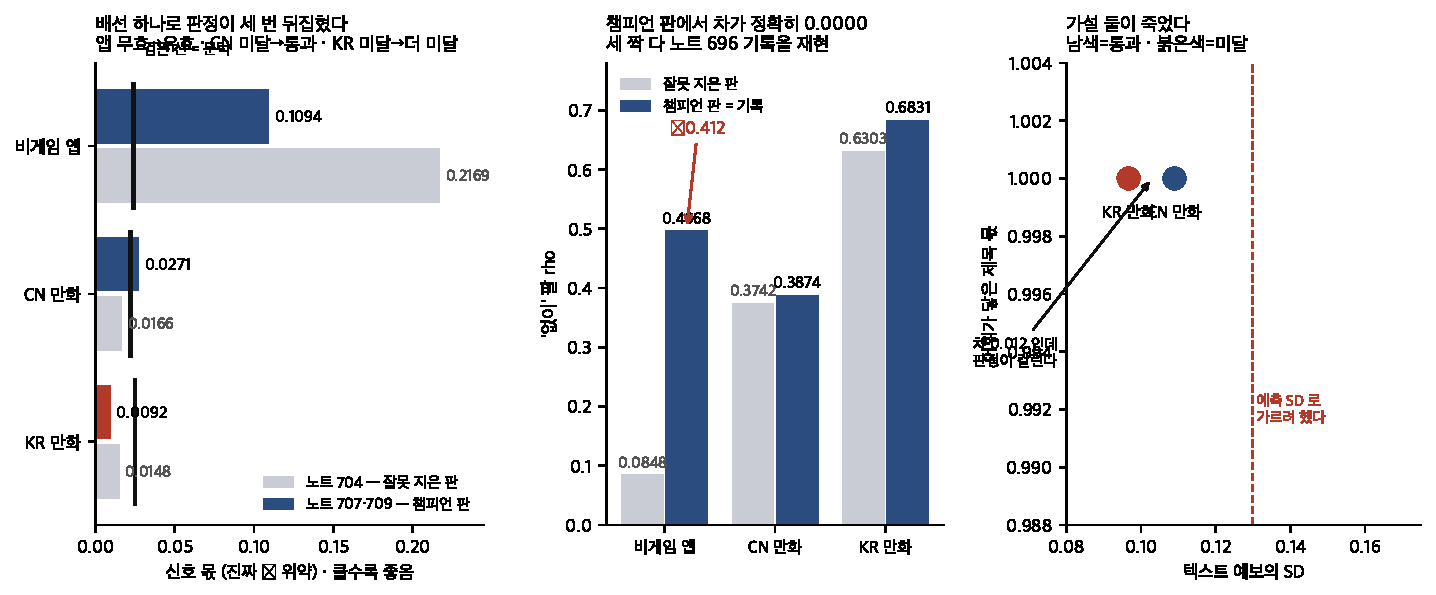
\includegraphics[width=0.99\textwidth]{figs/baseline.pdf}
\caption{왼쪽: 같은 열의 신호 몫이 두 판에서. \textbf{검은 선이 문턱이고 세 짝 다
판정이 바뀌었다.} 가운데: 챔피언 판에서 ``없이'' 팔이 기록과 \textbf{차 $0.0000$}.
오른쪽: 기제 가설 둘이 죽는 그림 --- 통과(남색)와 미달(붉은색)이 어느 축으로도
안 갈린다.}
\end{figure}

\begin{center}
\begin{tabular}{lrrrl}
\toprule
짝 & \multicolumn{2}{c}{``없이'' 팔 rho} & \multicolumn{2}{c}{신호 몫} \\
 & 잘못 지은 판 & 챔피언 판 & 노트 704 & 노트 707·709 \\
\midrule
비게임 앱 & $0.0848$ & $\mathbf{0.4968}$ & $0.2169$ \emph{무효} & $\mathbf{+0.1094}$ (4.6배) \\
CN 만화   & $0.3742$ & $\mathbf{0.3874}$ & $0.0166$ 미달 & $\mathbf{+0.0271}$ (1.23배) \\
KR 만화   & $0.6303$ & $\mathbf{0.6831}$ & $0.0148$ 미달 & $+0.0092$ (0.37배) \\
\bottomrule
\end{tabular}
\end{center}

챔피언 판에서 ``없이'' 팔이 \textbf{세 짝 다 노트 696 의 기록과 소수 넷째 자리까지
같다}($0.4968$ · $0.3874$ · $0.6831$, 차 $0.0000$). 그래서 오른쪽 두 열은 기록과 같은
자 위에 있다.

\claim{\textbf{잘못 지은 판 위에서 잰 증분은 ``챔피언 위에 더한 것''이 아니라
``빠진 축을 대신 메운 것''일 수 있다.} 앱에서 기준선이 $0.4968 \to 0.0848$ 로
$-0.412$ 무너졌고, 그 위에서 텍스트 열이 낸 $+0.2169$ 는 챔피언 판에서 $+0.1094$ 로
\textbf{절반이 됐다}. 무효였던 것은 \emph{크기}이고 \emph{존재}는 아니었다.}
{기준선이 무너진 판에서 잰 증분이 챔피언 판의 증분과 \emph{항상} 같은 부호라면 이
주장은 약해진다. 여기서는 세 짝 중 하나(KR)에서 부호는 같고 크기가 줄었고, 하나(CN)에서
크기가 늘었다 --- 방향이 일정하지 않다는 것이 오히려 근거다.}

\subsection*{그래서 관문을 코드에 넣었다}

노트 705 부터 러너가 \textbf{``없이'' 팔을 먼저 찍고, 기록 기준선의 $3\sigma$ 안에
안 오면 그 아래를 읽지 않고 멈춘다.} 노트 704 에서 문턱의 9배($0.2169$)를 하마터면
채택 후보로 올릴 뻔했고, 그때 막은 것은 코드가 아니라 우연히 기준선을 견줘 본 것이었다.

\section{내 예측이 두 번 다 틀렸다}

\begin{center}
\begin{tabular}{llll}
\toprule
 & 예측 & 결과 & \\
\midrule
노트 705 (앱) & 미달 · 순효과 음수 & $+0.1094$ · 순효과 $+0.0473$ & \textbf{둘 다 틀림} \\
노트 708 (KR) & $0.02$--$0.05$ 로 오름 & $+0.0092$ 로 \emph{내려감} & \textbf{틀림} \\
노트 708 (CN) & $0.01$--$0.04$ 미달 쪽 & $+0.0271$ \textbf{통과} & \textbf{틀림} \\
노트 708 (순효과) & 둘 다 양수로 & KR 만 음수로 남음 & \textbf{반만} \\
\bottomrule
\end{tabular}
\end{center}

노트 705 의 근거는 \emph{``노트 704 가 KR·CN 에서 순효과 음수를 봤고 그 기제가 앱에도
적용된다''} 였다. 노트 708 의 근거는 정반대로 \emph{``앱에서 강한 판 위에 텍스트가 더 잘
얹혔으니 만화도 그럴 것''} 이었다. \textbf{한 짝의 기제를 다른 짝으로 옮긴 추론이 두 번
연속 틀렸다.}

\claim{\textbf{짝 하나에서 얻은 기제를 다른 짝으로 옮기지 않는다.} 노트 551 · 560 ·
563 이 \emph{``전역 표의 도메인별 차로 처방을 만들지 말라''}를 세 번 적었고, 노트 678 이
그것을 단일 전환에서 확인했다. \textbf{이 논문이 네 번째 자리이고, 이번에는 도메인이
아니라 짝이다.}}
{짝이 넷 이상 생기고 기제가 재현되면 옮길 수 있다. 지금은 $n=3$ 이고 그중 둘이 같은
원천(만화)에서 나왔다.}

\section{기제 가설 둘이 죽었다}

노트 707 은 앱이 이긴 이유로 \textbf{어휘 겹침의 질}을 지목했다 --- 앱은 겹침
$0.98$ · 제목당 닿은 n-gram $19$ 인데 만화는 $1.00$ · $34$ 로, \emph{적게 닿는데
이긴다}. 그리고 예보 SD 가 앱 $0.158$ 대 만화 $0.097$ 로 갈리는 것을 곁증거로 봤다.

\textbf{KR 과 CN 이 그 둘을 다 죽였다.}

\begin{center}
\begin{tabular}{lrrrl}
\toprule
짝 & 겹침 & 닿은 n-gram & 예보 SD & 판정 \\
\midrule
비게임 앱 & $0.98$ & $19$ & $0.158$ & \textbf{통과} (4.6배) \\
CN 만화 & $1.00$ & $34$ & $0.109$ & \textbf{통과} (1.23배) \\
KR 만화 & $1.00$ & $35$ & $0.0967$ & 미달 (0.37배) \\
\bottomrule
\end{tabular}
\end{center}

CN 과 KR 은 겹침이 \textbf{똑같이 $1.00$} 이고 닿은 n-gram 이 $34$ 대 $35$ 다. 예보
SD 는 $0.109$ 대 $0.0967$ 로 \textbf{차가 $0.012$} 뿐인데 판정이 갈린다.
\textbf{그 폭으로 통과와 미달을 가를 수 없다.}

\subsection*{남는 가설 하나 --- 그리고 그것을 주장하지 않는 이유}

기준선이 높으면 얹을 자리가 없다. 실제로 \textbf{KR 이 기준선 최고($0.6831$)이고 신호
몫 최저($+0.0092$)}다. 그런데 앱($0.4968$)이 CN($0.3874$)보다 기준선이 높은데 신호 몫도
더 크다 --- \textbf{단조가 아니다.}

\claim{\textbf{$n=3$ 에서 순서를 맞히는 가설은 가설로만 적는다.} 세 점 중 둘이 같은
원천(만화)이고 하나가 단조를 깬다. 이 판은 같은 종류의 순서 관측을 세 번 처방으로
바꿨다가 세 번 틀렸다(551 · 560 · 563). \textbf{넷째 짝이 생길 때 시험한다.}}
{넷째 짝(예: JP 이외 애니, 비게임 앱의 다른 갈래)에서 기준선--신호몫 순서가 재현되면
가설이 산다. 재현 안 되면 여지 가설도 죽는다.}

\section{채택 상태 --- 셋 통과, 하나 미달, 하나 미측정}

\begin{center}
\begin{tabular}{lrrrl}
\toprule
자 & 신호 몫 & 문턱 & 배수 & \\
\midrule
판 & $+0.0119$ & $0.0045$ & $2.6\times$ & \textbf{통과} · 씨앗 12·40 재현 \\
비게임 앱 & $+0.1094$ & $0.024$ & $4.6\times$ & \textbf{통과} · 순효과 $+0.0473$ \\
CN 만화 & $+0.0271$ & $0.022$ & $1.23\times$ & \textbf{통과} · 순효과 $+0.0057$ \\
KR 만화 & $+0.0092$ & $0.025$ & $0.37\times$ & 미달 · \textbf{순효과 $-0.0042$} \\
날짜 통제 판 & --- & $0.0052$ & --- & \textbf{미측정} \\
\bottomrule
\end{tabular}
\end{center}

\textbf{채택하지 않는다.} 셋이 남았다. ① 다섯째 자를 안 쟀다. ② \textbf{CN 이 문턱의
$1.23$배}로 붙어 있고 씨앗 3 이라 얇다. ③ \textbf{KR 순효과가 음수}라 그 짝에서는 이
열이 해롭다 --- 채택하면 KR 성적이 내려가는 것을 감수하는 채택임을 명시해야 한다.

\claim{\textbf{다섯째 자는 판정을 못 바꾼다 --- 그것을 미리 적어 둔다.} 날짜 통제 판은
판과 상관 $+0.88$ 로 유효 독립 자 수를 $4.73/6$ 으로 떨어뜨린 \emph{바로 그} 붕괴한
방향이다(노트 629). 판이 $2.6$배로 통과했으므로 이것도 통과할 가능성이 높고,
\textbf{그 통과는 새 정보가 아니다.} 실제 판정을 가르는 것은 \textbf{CN 의 씨앗 확대}다.}
{날짜 통제 판이 \emph{미달}로 나오면 이 주장이 틀리고, 그것은 판과의 상관 $+0.88$ 이
이 축에서는 성립하지 않는다는 뜻이 된다 --- 그 자체로 값있는 결과다.}

\end{document}
